\section{Processi primari}
    \subsection{Accordo di fornitura}
    	In questo paragrafo vengono documentate le norme che i membri devono seguire affinché il gruppo possa diventare committente dei professori Vardanega e Cardin ed essere fornitori dell'azienda Zucchetti\pedice.
    \subsubsection{Studio di fattibilità}
        Dopo la presentazione dei capitolati il gruppo si è riunito per discutere la scelta più consona. Dopo aver risolto i dubbi interni ed aver redatto lo studio di fattibilità, documento, ad oggi \textit{in versione 1.0.0},  atto a valutare i pro e i contro di ogni progetto permettendo così una più attenta valutazione, si è optato per la scelta del capitolato \textit{numero 3}.  \newline
        I punti chiave dell'analisi sono i seguenti:
    	\begin{itemize}
		   \item \textbf{Introduzione:} Viene fatta una breve introduzione del contesto in cui applicare la soluzione;
		   \item \textbf{Finalità:} Viene descritto in modo sintetico lo scopo finale da raggiungere a lavoro completato;
		   \item \textbf{Tecnologie in uso:} Si descrivono genericamente i software che la proponente intende usare;
		   \item \textbf{Conclusioni:} Rappresenta il motivo per cui un capitolato è stato scelto oppure scartato.
	    \end{itemize}
    \subsubsection{Documentazione fornita}
	    Al fine di assicurare massima trasparenza e qualità alla proponente ed ai committenti verranno elencati i documenti forniti con una breve descrizione del loro contenuto:
    	\begin{itemize}
	        \item \textbf{Piano di progetto:} descrive la pianificazione, la consegna e il suo completamento;
	        \item \textbf{Analisi dei requisiti:} viene definita l'analisi dei casi d'uso e dei requisiti del gruppo
	        \item \textbf{Piano di qualifica:} verifica, validazione e garanzia della qualità dei processi e di prodotto.
	    \end{itemize}
    \newpage    
\subsection{Sviluppo}
    \subsubsection{Analisi dei requisiti}
    	L'Analisi dei Requisiti viene scritta dagli Analisti che hanno il compito di valutare in modo accurato ogni aspetto del progetto. In particolare questo documento è redatto con lo scopo di:
	    \begin{itemize}
	    	\item Descrivere scopo e funzionalità del prodotto;
	    	\item Fornire i requisiti e vincoli concordati col cliente;
	    	\item Descrivere gli elementi principali che hanno un ruolo chiave nello sviluppo del prodotto;
	    	\item Definire tutti i casi d'uso;
	    	\item Tracciare in modo dettagliato tutti i requisiti.\newline
	    \end{itemize}
    	L'Analisi dei Requisiti seguirà le specifiche descritte in seguito.\newline \newline
    	\textbf{Classificazione casi d'uso} Sono elencati in ordine dal più generico al più dettagliato ed è stato scelto il seguente criterio per la loro classificazione: \newline
	    \begin{center}
	    	UCX.Y
	    \end{center}
	    \begin{itemize}
	    	\item \textbf{Codice X:} E' il codice identificativo del caso d'uso generico che potrebbe suddividersi
	    	in casi d'uso più specifici. Nel caso non ci siano questi ultimi, il codice risulta univoco.
	    	\item \textbf{Codice Y:} E' un codice identificativo univoco per il caso d'uso. E' presente solo nel
	    	caso in cui il caso d'uso UCX abbia dei sotto casi d'uso più specifici.
	    \end{itemize}
	    X e Y sono numeri progressivi che stanno a indicare la specificità all'interno dei casi d'uso.\newline
	    Ogni caso d'uso è inoltre definito secondo la seguente struttura:\newline
	    \begin{itemize}
	    	\item \textbf{ID:} il codice del caso d'uso secondo la convenzione specificata poco sopra;
	    	\item \textbf{Nome:} titolo del caso d'uso;
	    	\item \textbf{Descrizione:} breve descrizione del caso d'uso;
	    	\item \textbf{Precondizione:} condizioni assunte come vere prima del verificarsi degli eventi del caso d'uso;
	    	\item \textbf{Postcondizione:} condizioni assunte come vere dopo il verificarsi degli eventi del caso d'uso;
	    	\item \textbf{Attori:} attori principali e secondari (se presenti) del caso d'uso;
	    	\item \textbf{Scenario Principale:} flusso degli eventi rappresentato attraverso una lista numerata.\newline
	    \end{itemize}
	    Nella \textit{Figura 1} viene riportato un esempio di caso d'uso:\newline \newline
    
	    \begin{figure}[!htbp]
	    	\centering
	    	
\includegraphics{casoduso.png}
	    	\caption{Esempio di caso d'uso}
	    \end{figure}
    
	    \textbf{Classificazione dei requisiti} Tutti i requisiti ottenuti dopo una profonda analisi degli Analisti possono essere ricavati da tre diverse fonti:\newline
	    \begin{itemize}
	    	\item \textbf{Interno:} il requisito proviene da una decisione del gruppo DreamCorp, generalmente emersa durante un incontro e riportata in un verbale;
	    	\item \textbf{Capitolato:} il requisito proviene dalle richieste del capitolato;
	    	\item \textbf{Esterno:} il requisito proviene da un incontro con la proponente.\newline
	    \end{itemize}
	    Il codice utilizzato per indicizzare univocamente i requisiti è il seguente:\newline
	    \begin{center}
	    	\textbf{R+(F|Q|V|P)+(C|O)+(X(.Y)*)}
	    \end{center}
	    \begin{itemize}
	    	\item \textbf{R:} Requisito;
	    	\item \textbf{F|Q|V|P:}
	    	\begin{itemize}
	    		\item F: Requisito funzionale che descrive nel dettaglio i servizi che verranno forniti dal sistema agli attori;
	    		\item Q: Requisito di qualità;
	    		\item V: Requisito di vincolo;
	    		\item P: Requisito prestazionale;
	    	\end{itemize}
	    	\item \textbf{C|O:}
	    	\begin{itemize}
	    		\item C: Compulsory (obbligatorio);
	    		\item O: Optional (opzionale);
	    	\end{itemize}
	    	\item \textbf{X.Y:} Numeri naturali concatenati con un punto per descrivere un sottorequisito.\newline
	    \end{itemize}
	    I requisiti di vincolo, di qualità e prestazionali fanno parte dei requisiti non funzionali che descrivono i vincoli sul sistema e sul suo processo di sviluppo.
	    Ad ogni requisito verranno infine associate la sua priorità, una breve descrizione e le sue fonti come nella \textit{Figura 2}.\newline
	    
	    \begin{figure}[!htbp]
	    	\centering
	    	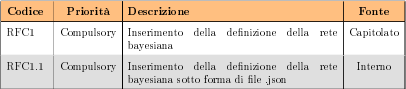
\includegraphics{requisiti.png}
	    	\caption{Esempio di requisito}
	    \end{figure}
	    
	    \textbf{Tracciamento} Infine, per facilitare la lettura e la visualizzazione dei requisiti, questi verranno indicizzati in due modalità specifiche:
	    \begin{itemize}
	    	\item \textbf{Tracciamento Priorità-Requisito:} il focus è orientato sulla priorità;
	    	\item \textbf{Tracciamento Tipologia-Requisito:}il focus è orientato sulla tipologia.\newline
	    \end{itemize}
	    Per una lettura immediata non sono riportate le descrizioni per le quali si rimanda alle sezioni apposite nel documento "Analisi dei Requisiti".
	    Infine viene riportata una tabella riassuntiva che permette di avere un quadro generale della distribuzione dei requisiti.\newline
\subsubsection{Qualità di Processo}
	    Per facilitare il tracciamento dei processi viene utilizzata una rappresentazione contratta formulata come segue:
	    \begin{center}
	    	\textbf{PX}
	    \end{center}
	    dove P sta per \textit{processo} e X è un numero intero progressivo.
\subsubsection{Qualità del software}
Per qualità del software si intende la misura in cui un prodotto software soddisfa un certo numero di aspettative rispetto sia al suo funzionamento che alla struttura interna. I parametri verranno classificati in:
\begin{itemize}
    \item{\textbf{Interni:} qualità percepita dagli sviluppatori;}
    \item{\textbf{Esterni:} qualità percepita dall'utente finale.}
\end{itemize}
Al fine di rendere piu' facile il tracciamento dei parametri viene utilizzata una codifica formulata come segue:
\begin{itemize}
    \item{\textbf{IX:} parametri interni;}
    \item{\textbf{EY:} parametri esterni.}
\end{itemize}
Dove X e Y sono numeri interi progressivi indipendenti.
	    \subsubsection{Progettazione}
	    L'attività di Progettazione consiste nel descrivere una soluzione al problema che sia soddisfacente per tutti gli stakeholders\pedice. Ciò serve a garantire che il prodotto sviluppato soddisfi le qualità, le proprietà e i bisogni nell'attività di analisi permettendo cosi di:
	    \begin{itemize}
	        \item Garantire la qualità del prodotto;
	        \item Ripartire il problema originale in maniera ricorsiva facilitando cosi la codifica delle componenti;
	        \item Ottimizzare.
	    \end{itemize}	
	    \textbf{Uso di diagrammi} Al fine di essere il più comprensibili possibile sarà necessario far uso su larga scala di diagrammi UML\pedice 2.0
	    \subsubsection{Codifica}
	In  questa  sotto-sezione  vengono  elencate  le  norme   alle  quali  i  Programmatori  devono attenersi durante l’attività di programmazione ed implementazione. Ogni  norma e'  rappresentata  da  un  paragrafo contenente un titolo,  una breve descrizione e, se necessario, un esempio esplicativo.  Alcune di esse possono anche contenere una lista di possibili eccezioni d’uso. L’uso di norme e convenzioni e' fondamentale per permettere la generazione di codice leggibile e uniforme, agevolare le fasi di manutenzione,  verifica e validazione e migliorare la qualità di prodotto. \newline
~\newline	
\textbf{Indentazione 1:} I blocchi innestati devono essere correttamente indentati usando quattro spazi per ciascun livello. \newline
	Esempio:\newline
	\begin{figure}[!htbp]
		\centering
		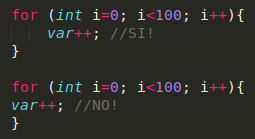
\includegraphics{indentazione1.png}
		\caption{Indentazione 1}
	\end{figure}
~\newline	
	\textbf{Indentazione 2:} E' vietato l'uso di tabulazioni che possono non essere uniformi tra diversi editor o IDE. Al loro posto vanno usati gli opportuni spazi. \newline
~\newline	
	\textbf{Indentazione 3:} Il codice che fa parte di un blocco deve essere innestato allo stesso livello di quel blocco. \newline
	Esempio:\newline
	\begin{figure}[!htbp]
		\centering
		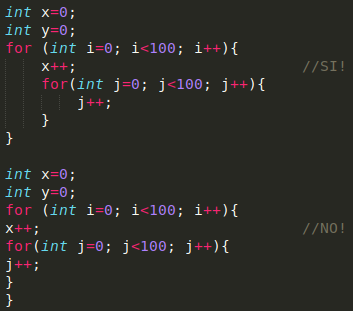
\includegraphics{indentazione3.png}
		\caption{Indentazione 3}
	\end{figure}
~\newline	
	\textbf{Parentesizzazione 1:} I blocchi di codice sono sempre racchiusi fra parentesi graffe.\newline 
	\textbf{Eccezione:} se il blocco e' composto da un'unica istruzione le parentesi possono essere omesse.\newline
	~\newline
	\textbf{Parentesizzazione 2:} Le parentesi graffe iniziano sempre nella stessa linea del codice. \newline
	~\newline
	\textbf{Nomenclatura:} Classi, metodi e variabili devono avere un nome univoco e quanto piu' descrittivo possibile. Inoltre devono rispettare le buone norme di scrittura in modo da distinguere immediatamente se si tratta di un nome di una classe, un metodo o una variabile. Nello specifico:\newline
	\begin{itemize}
	\item \textbf{Classi:} cominciano sempre con la lettera maiuscola;
	\item \textbf{Metodi:} cominciano sempre con una lettera minuscola e se sono composti da più parole le successive iniziano con una lettera maiuscola;
	\item \textbf{Variabili:} tutte le lettere sono minuscole ed e' consentito l'utilizzo del simbolo underscore "\_".\newline
	\end{itemize}
	La lingua utilizzata deve essere l'inglese.\newline
	~\newline
	\textbf{TODO:} Un commento TODO va utilizzato per descrivere codice non definitivo, migliorabile e per soluzioni a breve termine. Può essere anche usato per eventi futuri specificando accuratamente la data.\newline
	\textbf{Esempio:}\newline
	\begin{figure}[!htbp]
		\centering
		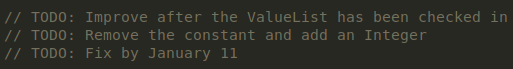
\includegraphics{todo.png}
		\caption{Esempi di TODO}
	\end{figure}
	~\newline
	\textbf{Visibilità:} Le variabili vanno dichiarate strettamente dove sono necessarie, ovvero nel blocco più interno che comprenda il loro utilizzo. Le variabili di ciclo vanno dichiarate nello statement a meno di una motivazione valida e opportunamente giustificata per non fare ciò. Le variabili globali vanno evitate in tutti i casi.\newline
	~\newline
	\textbf{Inizializzazione:} Le variabili vanno inizializzate il prima possibile, nel migliore dei casi subito dopo la loro dichiarazione. \newline
	~\newline
	\textbf{Lunghezza metodi e codice:} E' da evitare una lunghezza eccessiva sia nei metodi che nelle righe di codice. Nel primo caso una giusta suddivisione rende più manutenibili i vari metodi e più chiaro il loro scopo, nel secondo rende il codice più scorrevole \newline